
\documentclass[letterpaper,hide notes,xcolor={table,svgnames},pdftex,10pt]{beamer}
\def\showexamples{t}

\usecolortheme{crane}
\setbeamertemplate{navigation symbols}{}

\usetheme{MyPittsburgh}
\usepackage{hyperref}
\usepackage{graphicx,xspace}
\usepackage[normalem]{ulem}
\usepackage{multicol}
\usepackage{amsmath,amssymb,amsthm,graphicx,xspace}
\newcommand\SF[1]{$\bigstar$\footnote{SF: #1}}

\usepackage[sfdefault,lf]{carlito}
\usepackage[T1]{fontenc}
\usepackage[scaled]{beramono}
\usepackage{tikzpagenodes}
\newcommand{\Rplus}{\protect\hspace{-.1em}\protect\raisebox{.35ex}{\small{\small\textbf{+}}}}
\newcommand{\Cpp}{\mbox{C\Rplus\Rplus}\xspace}

\newcounter{tmpnumSlide}
\newcounter{tmpnumNote}

\newcommand\mnote[1]{%
	\addtocounter{tmpnumSlide}{1}
	\ifdefined\showcues {~\tiny\fbox{\arabic{tmpnumSlide}}}\fi
	\note{\setlength{\parskip}{1ex}\addtocounter{tmpnumNote}{1}\textbf{\Large \arabic{tmpnumNote}:} {#1\par}}}

\newcommand\mmnote[1]{\note{\setlength{\parskip}{1ex}#1\par}}


\newcommand\mquestion[2]{{~\color{red}\fbox{?}}\note{\setlength{\parskip}{1ex}\par{\Large \textbf{?}} #1} \note{\setlength{\parskip}{1ex}\par{\Large \textbf{A}} #2\par}\ifdefined \presentationonly \pause \fi}

\newcommand\blackboard[1]{%
	\ifdefined   \showblackboard
		{#1}
	\else {\begin{center} \fbox{\colorbox{blue!30}{%
						\begin{minipage}{.95\linewidth}%
							\hspace{\stretch{1}} Some space intentionally left blank; done at the blackboard.%
						\end{minipage}}}\end{center}}%
	\fi%
}

\usepackage{listings}
\lstset{%
	keywordstyle=\bfseries,
	aboveskip=15pt,
	belowskip=15pt,
	captionpos=b,
	identifierstyle=\ttfamily,
	frame=lines,
	numbers=left, basicstyle=\scriptsize, numberstyle=\tiny, stepnumber=0, numbersep=2pt}

\usepackage{siunitx}
\newcommand\sius[1]{\num[group-separator = {,}]{#1}\si{\micro\second}}
\newcommand\sims[1]{\num[group-separator = {,}]{#1}\si{\milli\second}}
\newcommand\sins[1]{\num[group-separator = {,}]{#1}\si{\nano\second}}
\sisetup{group-separator = {,}, group-digits = true}

%% -------------------- tikz --------------------
\usepackage{tikz}
\usetikzlibrary{positioning}
\usetikzlibrary{arrows,backgrounds,automata,decorations.shapes,decorations.pathmorphing,decorations.markings,decorations.text}

\tikzstyle{place}=[circle,draw=blue!50,fill=blue!20,thick, inner sep=0pt,minimum size=6mm]
\tikzstyle{transition}=[rectangle,draw=black!50,fill=black!20,thick, inner sep=0pt,minimum size=4mm]

\tikzstyle{block}=[rectangle,draw=black, thick, inner sep=5pt]
\tikzstyle{bullet}=[circle,draw=black, fill=black, thin, inner sep=2pt]

\tikzstyle{pre}=[<-,shorten <=1pt,>=stealth',semithick]
\tikzstyle{post}=[->,shorten >=1pt,>=stealth',semithick]
\tikzstyle{bi}=[<->,shorten >=1pt,shorten <=1pt, >=stealth',semithick]

\tikzstyle{mut}=[-,>=stealth',semithick]

\tikzstyle{treereset}=[dashed,->, shorten >=1pt,>=stealth',thin]

\usepackage{ifmtarg}
\usepackage{xifthen}
\makeatletter
% new counter to now which frame it is within the sequence
\newcounter{multiframecounter}
% initialize buffer for previously used frame title
\gdef\lastframetitle{\textit{undefined}}
% new environment for a multi-frame
\newenvironment{multiframe}[1][]{%
	\ifthenelse{\isempty{#1}}{%
		% if no frame title was set via optional parameter,
		% only increase sequence counter by 1
		\addtocounter{multiframecounter}{1}%
	}{%
		% new frame title has been provided, thus
		% reset sequence counter to 1 and buffer frame title for later use
		\setcounter{multiframecounter}{1}%
		\gdef\lastframetitle{#1}%
	}%
	% start conventional frame environment and
	% automatically set frame title followed by sequence counter
	\begin{frame}%
		\frametitle{\lastframetitle~{\normalfont(\arabic{multiframecounter})}}%
		}{%
	\end{frame}%
}
\makeatother

\makeatletter
\newdimen\tu@tmpa%
\newdimen\ydiffl%
\newdimen\xdiffl%
\newcommand\ydiff[2]{%
	\coordinate (tmpnamea) at (#1);%
	\coordinate (tmpnameb) at (#2);%
	\pgfextracty{\tu@tmpa}{\pgfpointanchor{tmpnamea}{center}}%
	\pgfextracty{\ydiffl}{\pgfpointanchor{tmpnameb}{center}}%
	\advance\ydiffl by -\tu@tmpa%
}
\newcommand\xdiff[2]{%
	\coordinate (tmpnamea) at (#1);%
	\coordinate (tmpnameb) at (#2);%
	\pgfextractx{\tu@tmpa}{\pgfpointanchor{tmpnamea}{center}}%
	\pgfextractx{\xdiffl}{\pgfpointanchor{tmpnameb}{center}}%
	\advance\xdiffl by -\tu@tmpa%
}
\makeatother
\newcommand{\copyrightbox}[3][r]{%
	\begin{tikzpicture}%
		\node[inner sep=0pt,minimum size=2em](ciimage){#2};
		\usefont{OT1}{phv}{n}{n}\fontsize{4}{4}\selectfont
		\ydiff{ciimage.south}{ciimage.north}
		\xdiff{ciimage.west}{ciimage.east}
		\ifthenelse{\equal{#1}{r}}{%
			\node[inner sep=0pt,right=1ex of ciimage.south east,anchor=north west,rotate=90]%
			{\raggedleft\color{black!50}\parbox{\the\ydiffl}{\raggedright{}#3}};%
		}{%
			\ifthenelse{\equal{#1}{l}}{%
				\node[inner sep=0pt,right=1ex of ciimage.south west,anchor=south west,rotate=90]%
				{\raggedleft\color{black!50}\parbox{\the\ydiffl}{\raggedright{}#3}};%
			}{%
				\node[inner sep=0pt,below=1ex of ciimage.south west,anchor=north west]%
				{\raggedleft\color{black!50}\parbox{\the\xdiffl}{\raggedright{}#3}};%
			}
		}
	\end{tikzpicture}
}


%% --------------------

%\usepackage[excludeor]{everyhook}
%\PushPreHook{par}{\setbox0=\lastbox\llap{MUH}}\box0}

%\vspace*{\stretch{1}

%\setbox0=\lastbox \llap{\textbullet\enskip}\box0}

\setlength{\parskip}{\fill}

\newcommand\noskips{\setlength{\parskip}{1ex}}
\newcommand\doskips{\setlength{\parskip}{\fill}}

\newcommand\xx{\par\vspace*{\stretch{1}}\par}
\newcommand\xxs{\par\vspace*{2ex}\par}
\newcommand\tuple[1]{\langle #1 \rangle}
\newcommand\code[1]{{\sf \footnotesize #1}}
\newcommand\ex[1]{\uline{Example:} \ifdefined \presentationonly \pause \fi
	\ifdefined\showexamples#1\xspace\else{\uline{\hspace*{2cm}}}\fi}

\newcommand\ceil[1]{\lceil #1 \rceil}


\AtBeginSection[]
{
	\begin{frame}
		\frametitle{Outline}
		\tableofcontents[currentsection]
	\end{frame}
}



\pgfdeclarelayer{edgelayer}
\pgfdeclarelayer{nodelayer}
\pgfsetlayers{edgelayer,nodelayer,main}

\tikzstyle{none}=[inner sep=0pt]
\tikzstyle{rn}=[circle,fill=Red,draw=Black,line width=0.8 pt]
\tikzstyle{gn}=[circle,fill=Lime,draw=Black,line width=0.8 pt]
\tikzstyle{yn}=[circle,fill=Yellow,draw=Black,line width=0.8 pt]
\tikzstyle{empty}=[circle,fill=White,draw=Black]
\tikzstyle{bw} = [rectangle, draw, fill=blue!20,
text width=4em, text centered, rounded corners, minimum height=2em]

\newcommand{\CcNote}[1]{% longname
	This work is licensed under the \textit{Creative Commons #1 3.0 License}.%
}
\newcommand{\CcImageBy}[1]{%
	\includegraphics[scale=#1]{creative_commons/cc_by_30.pdf}%
}
\newcommand{\CcImageSa}[1]{%
	\includegraphics[scale=#1]{creative_commons/cc_sa_30.pdf}%
}
\newcommand{\CcImageNc}[1]{%
	\includegraphics[scale=#1]{creative_commons/cc_nc_30.pdf}%
}
\newcommand{\CcGroupBySa}[2]{% zoom, gap
	\CcImageBy{#1}\hspace*{#2}\CcImageNc{#1}\hspace*{#2}\CcImageSa{#1}%
}
\newcommand{\CcLongnameByNcSa}{Attribution-NonCommercial-ShareAlike}

\newenvironment{changemargin}[1]{% 
	\begin{list}{}{% 
		\setlength{\topsep}{0pt}% 
		\setlength{\leftmargin}{#1}% 
		\setlength{\rightmargin}{1em}
		\setlength{\listparindent}{\parindent}% 
		\setlength{\itemindent}{\parindent}% 
		      \setlength{\parsep}{\parskip}% 
		      }% 
		\item[]}{\end{list}}




\title{Lecture 7 --- Sockets }

\author{Jeff Zarnett \\ \small \texttt{jzarnett@uwaterloo.ca}}
\institute{Department of Electrical and Computer Engineering \\
	University of Waterloo}
\date{\today}


\begin{document}

\begin{frame}
	\titlepage

\end{frame}


\begin{frame}
	\frametitle{Network Communication}

	\begin{center}
		
\includegraphics[width=0.7\textwidth]{images/seriesoftubes.jpg}\\
		Former US Senator Ted Stevens
	\end{center}


\end{frame}


\begin{frame}
	\frametitle{Network Communication}

	If two processes aren't on the same machine, we need to use the network.

	The network is frequently portrayed as a mysterious cloud blob:

	\begin{center}
		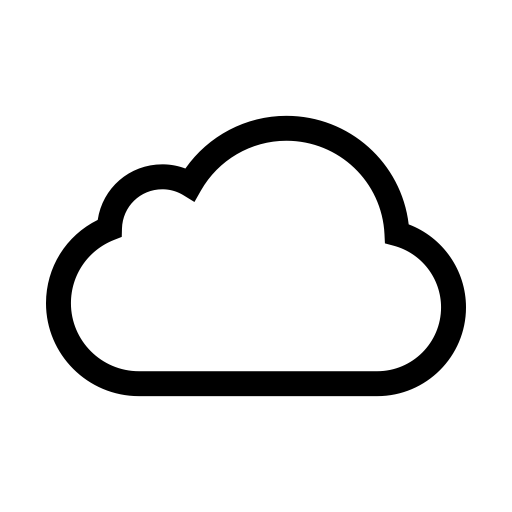
\includegraphics[width=0.35\textwidth]{images/iCloud.png}\\
		The Apple iCloud icon
	\end{center}

\end{frame}


\begin{frame}
	\frametitle{The Socket}

	The \alert{socket} API describes how to communicate over the network.

	The socket is the concept for how to establish a communication channel.

	There are two ways we can communicate: datagrams and connection streams.

	\begin{center}
		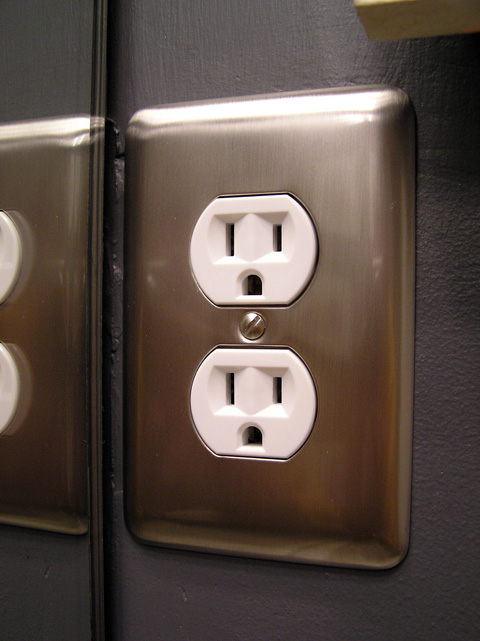
\includegraphics[width=0.3\textwidth]{images/electrical-outlet.jpg}
	\end{center}

\end{frame}


\begin{frame}
	\frametitle{Call or Text?}

	The connection stream is like a telephone call.

	Both parties have to be on the line to communicate.

	Datagram is like texting or sending a letter in the mail.

	Datagrams are unidirectional and can get lost!


\end{frame}

\begin{frame}[fragile]
	\frametitle{Sockets are Files}

	Much like everything else in UNIX, a socket is handled like a file.

	To create a socket, we need the \texttt{sys/socket.h} header

	\begin{lstlisting}[language=C]
int socket( int domain, int type, int protocol )
\end{lstlisting}

	Domain: address format; \texttt{AF\_INET} (IPv4)

	Type: what kind of data; \texttt{SOCK\_DGRAM} or\texttt {SOCK\_STREAM}

	Protocol: how data is transported; 0 for default (TCP/IP).

\end{frame}


\begin{frame}
	\frametitle{Check the Boot of the Car for your Jumper}

	Speaking the same dialect is important.

	Consider a 4-byte integer. Two possible organizations:

	\begin{center}
		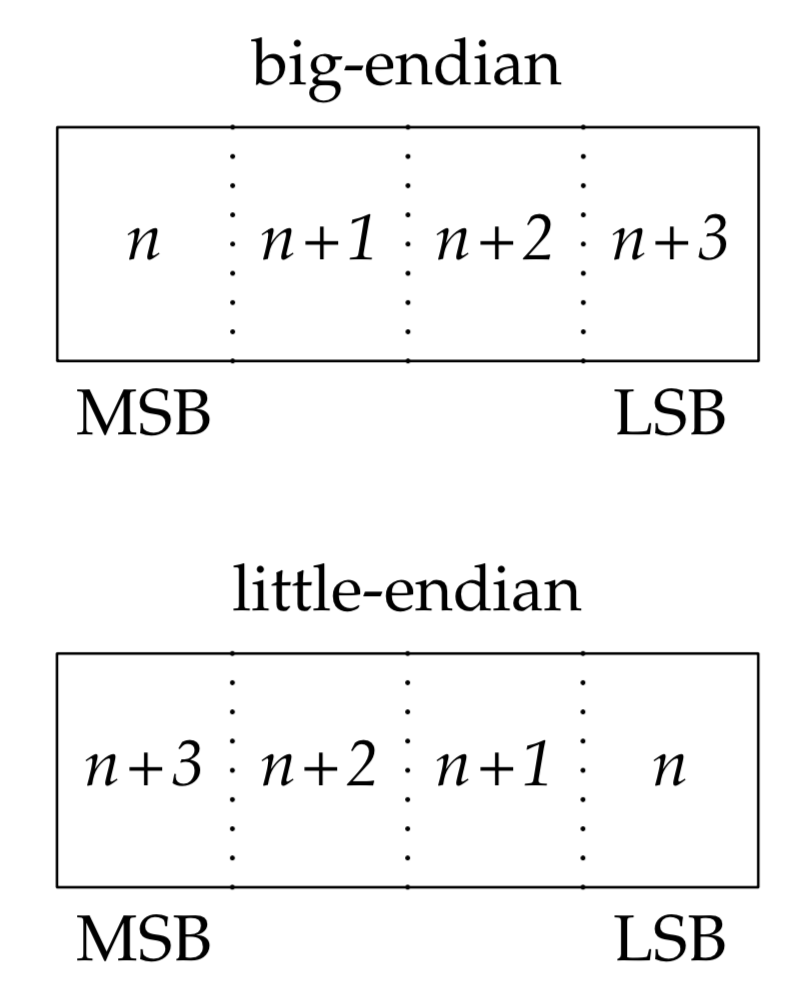
\includegraphics[width=0.25\textwidth]{images/endian}
	\end{center}

	Network protocol specifies the use of big-endian!

\end{frame}


\begin{frame}[fragile]
	\frametitle{Translate!}

	Included in the \texttt{arpa/inet.h} header are some functions to help us out.

	Their use is advisable even if you're sure the system you are using is big-endian, because of portability of your code.

	\begin{lstlisting}[language=C]
uint32_t htonl( uint32_t hostint32 ) /* Translate 4 byte int to network format */
uint16_t htons( uint16_t hostint16 ) /* Translate 2 byte int to network format */
uint32_t ntohl( uint32_t netint32 )  /* Translate 4 byte int to host format */
uint16_t ntohs( uint16_t netint16 ) /* Translate 2 byte int to host format */
\end{lstlisting}


\end{frame}


\begin{frame}[fragile]
	\frametitle{An Internet Address}

	When we want to call someone, we have to put in their phone number.

	If we want someone to call us, we need a phone number and we need to be ready to receive calls.

	An internet address is represented by the following structure:
	\begin{lstlisting}[language=C]
struct sockaddr_in {
  sa_family_t sin_family; /* Address family */
  in_port_t sin_port; /* Port number */
  struct in_addr sin_addr; /* IPv4 Address */
};
\end{lstlisting}

\end{frame}


\begin{frame}[fragile]
	\frametitle{Initializing an Address}

	\begin{lstlisting}[language=C]
struct sockaddr_in addr;
addr.sin_family = AF_INET;
addr.sin_port = htons( 2520 );
addr.sin_addr.s_addr = htonl( INADDR_ANY );
\end{lstlisting}

	\texttt{AF\_INET} is IPv4.

	You are probably quite familiar with how they look: 192.168.0.1

	But if you want to go to uwaterloo.ca a translation to an IP address takes place.

	Here we chose a constant value, \texttt{INADDR\_ANY}\\
	\quad Choose an address of the current computer.

\end{frame}


\begin{frame}
	\frametitle{Ports: Like Apartments!}

	Imagine your computer is then an apartment building; the port number is which apartment the connection is made with.

	Different services (processes) are communicating over different ports.

	No two processes can be using the same port at the same time.

	By convention, ports with numbers below 1024 considered to be reserved for system services.

	Example: \texttt{ssh} on port 22.

\end{frame}


\begin{frame}
	\frametitle{Address Lookup}

	\begin{center}
		
\includegraphics[width=0.6\textwidth]{images/terminator-phonebook1.jpg}
	\end{center}
	\begin{center}
		
\includegraphics[width=0.6\textwidth]{images/terminator-phonebook2.jpg}
	\end{center}


\end{frame}


\begin{frame}
	\frametitle{Address Lookup}

	We probably only rarely use IP addresses directly; we use human-friendly names.

	For example, you use \texttt{ssh username@ecelinux.uwaterloo.ca} and don't need to manually look up the IP address for the server.

	Looking up hostnames and the like is somewhat complex (and not the focus), so we will just learn one method for doing this.

	Many examples and older texts use the function \texttt{gethostbyname()}, but this is now deprecated.

\end{frame}


\begin{frame}[fragile]
	\frametitle{Get Address Info!}

	The function is prototyped in in \texttt{netdb.h}:

	\begin{lstlisting}[language=C]
int getaddrinfo(const char *node,     // e.g. "www.example.com" or IP
                const char *service,  // e.g. "http" or port number
                const struct addrinfo *hints,
                struct addrinfo **res);
\end{lstlisting}

	\texttt{node}: hostname or IP address.

	\texttt{service}: protocol or port number.

	\texttt{hints}: used to restrict the kind of connection you want.

	\texttt{res}: pointer to be updated with the result.

\end{frame}


\begin{frame}[fragile]
	\frametitle{Look Up an Address Example}

	\begin{lstlisting}[language=C]
struct addrinfo hints;
struct addrinfo *serverinfo;  // will point to the results

memset(&hints, 0, sizeof hints); // make sure the struct is empty
hints.ai_family = AF_INET;     // Choose IPv4
hints.ai_socktype = SOCK_STREAM; // TCP stream sockets
hints.ai_flags = AI_PASSIVE;     // fill in my IP for me

int result = getaddrinfo("www.example.com", "2520", &hints, &serverinfo);
if (result != 0) {
  return -1;
}
struct sockaddr_in * sain = (struct sockaddr_in*) serverinfo->ai_addr;
/* Do things with this */

freeaddrinfo( serverinfo );
\end{lstlisting}


	Assuming that all went well, the \texttt{serverinfo} pointer is now pointing to a linked list of \texttt{struct sockaddr}.

	Most of the time we just need the first result.
\end{frame}


\begin{frame}
	\frametitle{Uh, where am I again?}

	If we are interested in getting the structure for the local computer, we can manually initialize the \texttt{struct sockaddr\_in} as we did earlier.

	Or we can call \texttt{getaddrinfo()} with \texttt{NULL} as the \texttt{node} parameter.

	It's possible to use \texttt{NULL} for the hints if you are willing to accept the defaults

	To deallocate the information that has been allocated, use \texttt{freeaddrinfo()}.
\end{frame}


\begin{frame}
	\frametitle{If you find a fork in the road... keep it}

	Up until now what we've learned applies to both the client and server side.

	Now the paths diverge.

	If we are the client, we'd like to connect to a server.

	This is the easier workflow. We just call \texttt{connect()}.

\end{frame}


\begin{frame}[fragile]
	\frametitle{Connect}

	\begin{lstlisting}[language=C]
int connect( int sockfd, struct sockaddr *addr, socklen_t len); 
\end{lstlisting}

	\texttt{sockfd}: the socket file descriptor (the \texttt{int} we got back from the call to \texttt{socket}).

	\texttt{addr}: address structure from our lookup.

	\texttt{len}: size of the address structure. \\
	\quad Use either \texttt{sizeof} or \texttt{ai\_addrlen}.

\end{frame}


\begin{frame}[fragile]
	\frametitle{Connect Example}

	\begin{lstlisting}[language=C]
struct addrinfo hints;
struct addrinfo *res;
int sockfd;

memset(&hints, 0, sizeof( hints ));
hints.ai_family = AF_INET;
hints.ai_socktype = SOCK_STREAM;

getaddrinfo("www.uwaterloo.ca", "80", &hints, &res);
sockfd = socket(res->ai_family, res->ai_socktype, res->ai_protocol);

int status = connect(sockfd, res->ai_addr, res->ai_addrlen);
\end{lstlisting}

	The return value (\texttt{status}) tells us if we were successful.

	0 indicates success.

	Check codes by looking at the man pages: \url{http://man7.org/linux/man-pages/man2/connect.2.html}

	Success means we're ready to communicate!

\end{frame}




\begin{frame}
	\frametitle{Server: Bind, Listen, Accept}


	The overview of what steps the server is going to do is bind, listen, and accept.

	The bind step is how we choose what port we are going to connect to.

	The listen step is the part where we wait for connections from a client.

	Then the last step is accept: establish the connection so we can start talking.

\end{frame}


\begin{frame}
	\frametitle{Bind, Listen, Accept}

	\begin{center}
		
\includegraphics[width=0.5\textwidth]{images/cheezburger.jpeg}
	\end{center}

\end{frame}


\begin{frame}[fragile]
	\frametitle{Bind}

	\texttt{bind()}: associate the socket with whatever port we want to use.

	When the \texttt{ssh} daemon is available for connection, it's because it has bound itself to the port 22 using \texttt{bind}.

	\begin{lstlisting}[language=C]
int socketfd = socket( AF_INET, SOCK_STREAM, 0 );
struct sockaddr_in addr;
addr.sin_family = AF_INET;
addr.sin_port = htons( 2520 );
addr.sin_addr.s_addr = htonl( INADDR_ANY );

bind( socketfd, (struct sockaddr*) &addr, sizeof( addr ));
\end{lstlisting}

	With that done, we've acquired the resource of port 2520 for our use.

\end{frame}


\begin{frame}
	\frametitle{Client Side Port?}

	You'll notice also \texttt{bind()} did not happen on the client side.

	This is because we don't care on the client side what the outgoing port number is.

	So we can just skip that step, unless we have a reason to care.

\end{frame}


\begin{frame}[fragile]
	\frametitle{Listen}

	\texttt{listen()}: int this step we wait for incoming connections.

	This is the simplest step and you just call:

	\begin{lstlisting}[language=C]
int listen(int sockfd, int backlog); 
\end{lstlisting}

	We listen on a socket that has been bound with \texttt{bind} and we'll allow a backlog up to \texttt{backlog} connections.

	If the queue is full the server system will reject additional requests.


\end{frame}


\begin{frame}[fragile]
	\frametitle{Acceptance is the Last Stage}

	So we've chosen a socket (got a phone number).

	We've said we're ready to listen (our phone is turned on).

	The next step is to \texttt{accept()} incoming \texttt{connect} requests (press the green icon).

	\begin{lstlisting}[language=C]
int accept( int sockfd, struct sockaddr *addr, socklen_t *len ); 
\end{lstlisting}

	The first parameter is, of course, the socket that we are listening to.

	The second and third parameters are the information about the client. We allocate these, pass them in, and they are updated by the call to \texttt{accept}.

	If we don't care at all about who the client is you can give in \texttt{NULL}.

\end{frame}


\begin{frame}
	\frametitle{Accept: ``Always Two, There Are''}

	The return value is a new file descriptor which describes a new socket.

	Further communication takes places over that socket (and not the original one).

	The original socket is still used for accepting connections, and the new one is the socket used for communication with the client.

	If \texttt{accept} is called and no requests are in the queue, the server is blocked until a request arrives. We simply wait for the connection.

\end{frame}


\begin{frame}[fragile]
	\frametitle{Put the Pieces Together}

	\begin{lstlisting}[language=C]
struct sockaddr_in client_addr;
int client_addr_size = sizeof( struct sockaddr_in );
int newsockfd;

int socketfd = socket( AF_INET, SOCK_STREAM, 0 );
struct sockaddr_in server_addr;
server_addr.sin_family = AF_INET;
server_addr.sin_port = htons( 2520 );
server_addr.sin_addr.s_addr = htonl( INADDR_ANY );

bind( socketfd, (struct sockaddr*) &server_addr, sizeof( server_addr ));
listen( socketfd, 5 );
newsockfd = accept( socktfd, (struct sockaddr*) &client_addr, &client_addr_size );

/* Do something useful */

close( newsockfd );

/* Later when all is done */
close( socketfd );
\end{lstlisting}
\end{frame}


\begin{frame}
	\frametitle{Acceptance is Ongoing}

	Unless communication is a one-time thing, we call \texttt{accept} in some sort of loop.

	We then are constantly accepting new connections and doing something useful with each, before going on to the next.

\end{frame}


\begin{frame}[fragile]
	\frametitle{Blocked Number}

	We could save ourselves some trouble by not caring about the client address:

	\begin{lstlisting}[language=C]
int newsockfd;

int socketfd = socket( AF_INET, SOCK_STREAM, 0 );
struct sockaddr_in server_addr;
server_addr.sin_family = AF_INET;
server_addr.sin_port = htons( 2520 );
server_addr.sin_addr.s_addr = htonl( INADDR_ANY );

bind( socketfd, (struct sockaddr*) &server_addr, sizeof( server_addr ));
listen( socketfd, 5 );
newsockfd = accept( socktfd, NULL, NULL );
/* Do something useful */

close( newsockfd );

/* Later when all is done */
close( socketfd );
\end{lstlisting}



\end{frame}


\begin{frame}
	\frametitle{Connection Established}

	\begin{center}
		
\includegraphics[width=0.7\textwidth]{images/data-connection.jpg}
	\end{center}

	We are finally ready for the client and server to communicate.

\end{frame}


\begin{frame}[fragile]
	\frametitle{Connection Established}

	The client communicates using its original socket file descriptor.

	The server communicates using the new file descriptor.

	Likely you will move some of the boilerplate into your own function, e.g.:

	\begin{lstlisting}[language=C]
int connect_to( const char* host, const char* port ); 
\end{lstlisting}

	Next: let's actually communicate!

\end{frame}


\end{document}

